\documentclass[11pt,letterpaper]{article}

\usepackage[T1]{fontenc}
\usepackage[utf8]{inputenc}
\usepackage{lmodern}
\usepackage{textcomp}
\usepackage[margin=1in]{geometry}
\usepackage{microtype}
\usepackage{amsmath,amssymb}
\usepackage{graphicx}
\usepackage{float}
\usepackage{booktabs}
\usepackage{array}
\usepackage{tabularx}
\usepackage{multirow}
\usepackage{xcolor}
\usepackage{url}
\usepackage[numbers,sort&compress]{natbib}
\usepackage[colorlinks=true,linkcolor=blue!50!black,citecolor=blue!50!black,
            urlcolor=blue!50!black,breaklinks=true]{hyperref}

\graphicspath{{figures/}}

% caption.sty is unavailable in this TeX installation; this reproduces the
% journal-style caption (bold label, small text) from the LaTeX kernel.
\makeatletter
\long\def\@makecaption#1#2{%
  \vskip\abovecaptionskip
  \sbox\@tempboxa{\small\textbf{#1.} #2}%
  \ifdim\wd\@tempboxa>\hsize
    {\small\textbf{#1.} #2\par}%
  \else
    \global\@minipagefalse
    \hb@xt@\hsize{\hfil\box\@tempboxa\hfil}%
  \fi
  \vskip\belowcaptionskip}
\makeatother

\newcommand{\Fio}{FiO$_2$}
\newcommand{\Spo}{SpO$_2$}

\title{\bfseries Can published ARDS subphenotype classifiers survive\\
routine ICU data?\\[0.35em]
\large A reproduction and deployment stress-test across six open datasets}
\author{James Conde}
\date{2026}

\begin{document}
\maketitle

\begin{abstract}
\noindent
\textbf{Background.} The hyperinflammatory and hypoinflammatory subphenotypes of the acute
respiratory distress syndrome are established and independently replicated, and have been
reduced to parsimonious classifiers intended for bedside use. Every published validation of
those classifiers, however, has run in curated research cohorts, where variables were
measured on protocol and missingness was low by design. Whether they survive routine care
is untested.

\textbf{Methods.} Six open datasets, three modalities. A reference two-class assignment was
derived by Gaussian mixture on 4,680 patients from one hospital system of the
PhysioNet/CinC Challenge 2019 corpus, then reproduced by classifiers restricted to
per-patient values and verified portable by two independent checks. The frozen models were
applied to a second hospital system, and to the eICU demonstration database under an
entirely different schema. A modified SOFA score, a variable-ablation curve, a prognostic
enrichment simulation and one iterative refinement cycle were pre-specified. A molecular
layer used three transcriptomic cohorts and a 1,472-assay proteomic cohort.

\textbf{Results.} The expected two-class directional pattern was recovered at 28.5\,\%
prevalence, and portable classifiers reproduced that reference assignment
($\kappa = 0.852$). Transfer was limited not by the model but by measurement: the
frozen classifier scored 82.4\,\% of second-hospital patients using coverage-matched
variables and 1.6\,\% using the variables that performed best, because bicarbonate is
charted for 97.4\,\% of patients at one site and 2.1\,\% at the other. Expressed as trial
screening burden, this is a 52-fold difference. Against sepsis onset the classes appeared
near-worthless, adding $+0.017$ AUC over a severity score; against mortality in eICU the
same frozen model separated 16.8\,\% from 36.6\,\% hospital mortality ($p < 0.0001$).

\textbf{Conclusion.} Reproducibility, portability and deployability are distinct
properties. A classifier can recover a published structure, run without cohort-derived
preprocessing, and still be unusable at another hospital because the measurements it
requires are not routinely obtained. The apparent weakness of the classes on the primary
cohort depended strongly on the available endpoint.
\end{abstract}

\section{Introduction}

Latent class analysis of two randomised trials identified two inflammatory subphenotypes of
ARDS \citep{calfee2014}, a finding since recovered across five or more cohorts and shown to
carry differential mortality \citep{famous2017} and differential treatment response.
Subsequent work reduced the classification to parsimonious models usable from routinely
available data \citep{sinha2020lrm,sinha2020ajrccm}, and validated those models in
observational cohorts \citep{sinha2022}. \textbf{This study reproduces that established
structure; it does not discover it.} Any reading of what follows as a novel finding about
subphenotype existence would be a misreading.

What remains open is deployability. The validations above ran in ARDSNet trials, EARLI,
VALID and LUNG SAFE --- cohorts in which the classifier's input variables were measured on
protocol. Routine intensive care is not like that. Laboratory measurement is intermittent,
ordering behaviour differs between institutions, and missingness in electronic health
records is well established as informative rather than random, reflecting care process
rather than patient biology alone.

\textbf{Three properties are conflated in most of this literature, and this study
separates them.} \emph{Reproducibility} is whether a published structure can be recovered in
a new dataset. \emph{Portability} is whether a model can run without cohort-derived
preprocessing --- no z-scores against a population, no median imputation.
\emph{Deployability} is whether the measurements the model requires are actually obtained at
the site where it would run. A classifier can satisfy the first two completely and fail the
third, and the third is where this study's contribution lies.

This gives a concrete operational question, and it is the question a clinical-development
team faces when designing an enrichment strategy: \emph{do published subphenotype
classifiers survive routine, sparsely measured, unadjudicated ICU data, and how gracefully
do they degrade as the variables they need go missing?}

The study is deliberately constrained to open-access data. That costs real capability ---
most consequentially, the primary cohort has no mortality outcome --- and buys schedule
certainty and full reproducibility.

\begin{figure}[H]
  \centering
  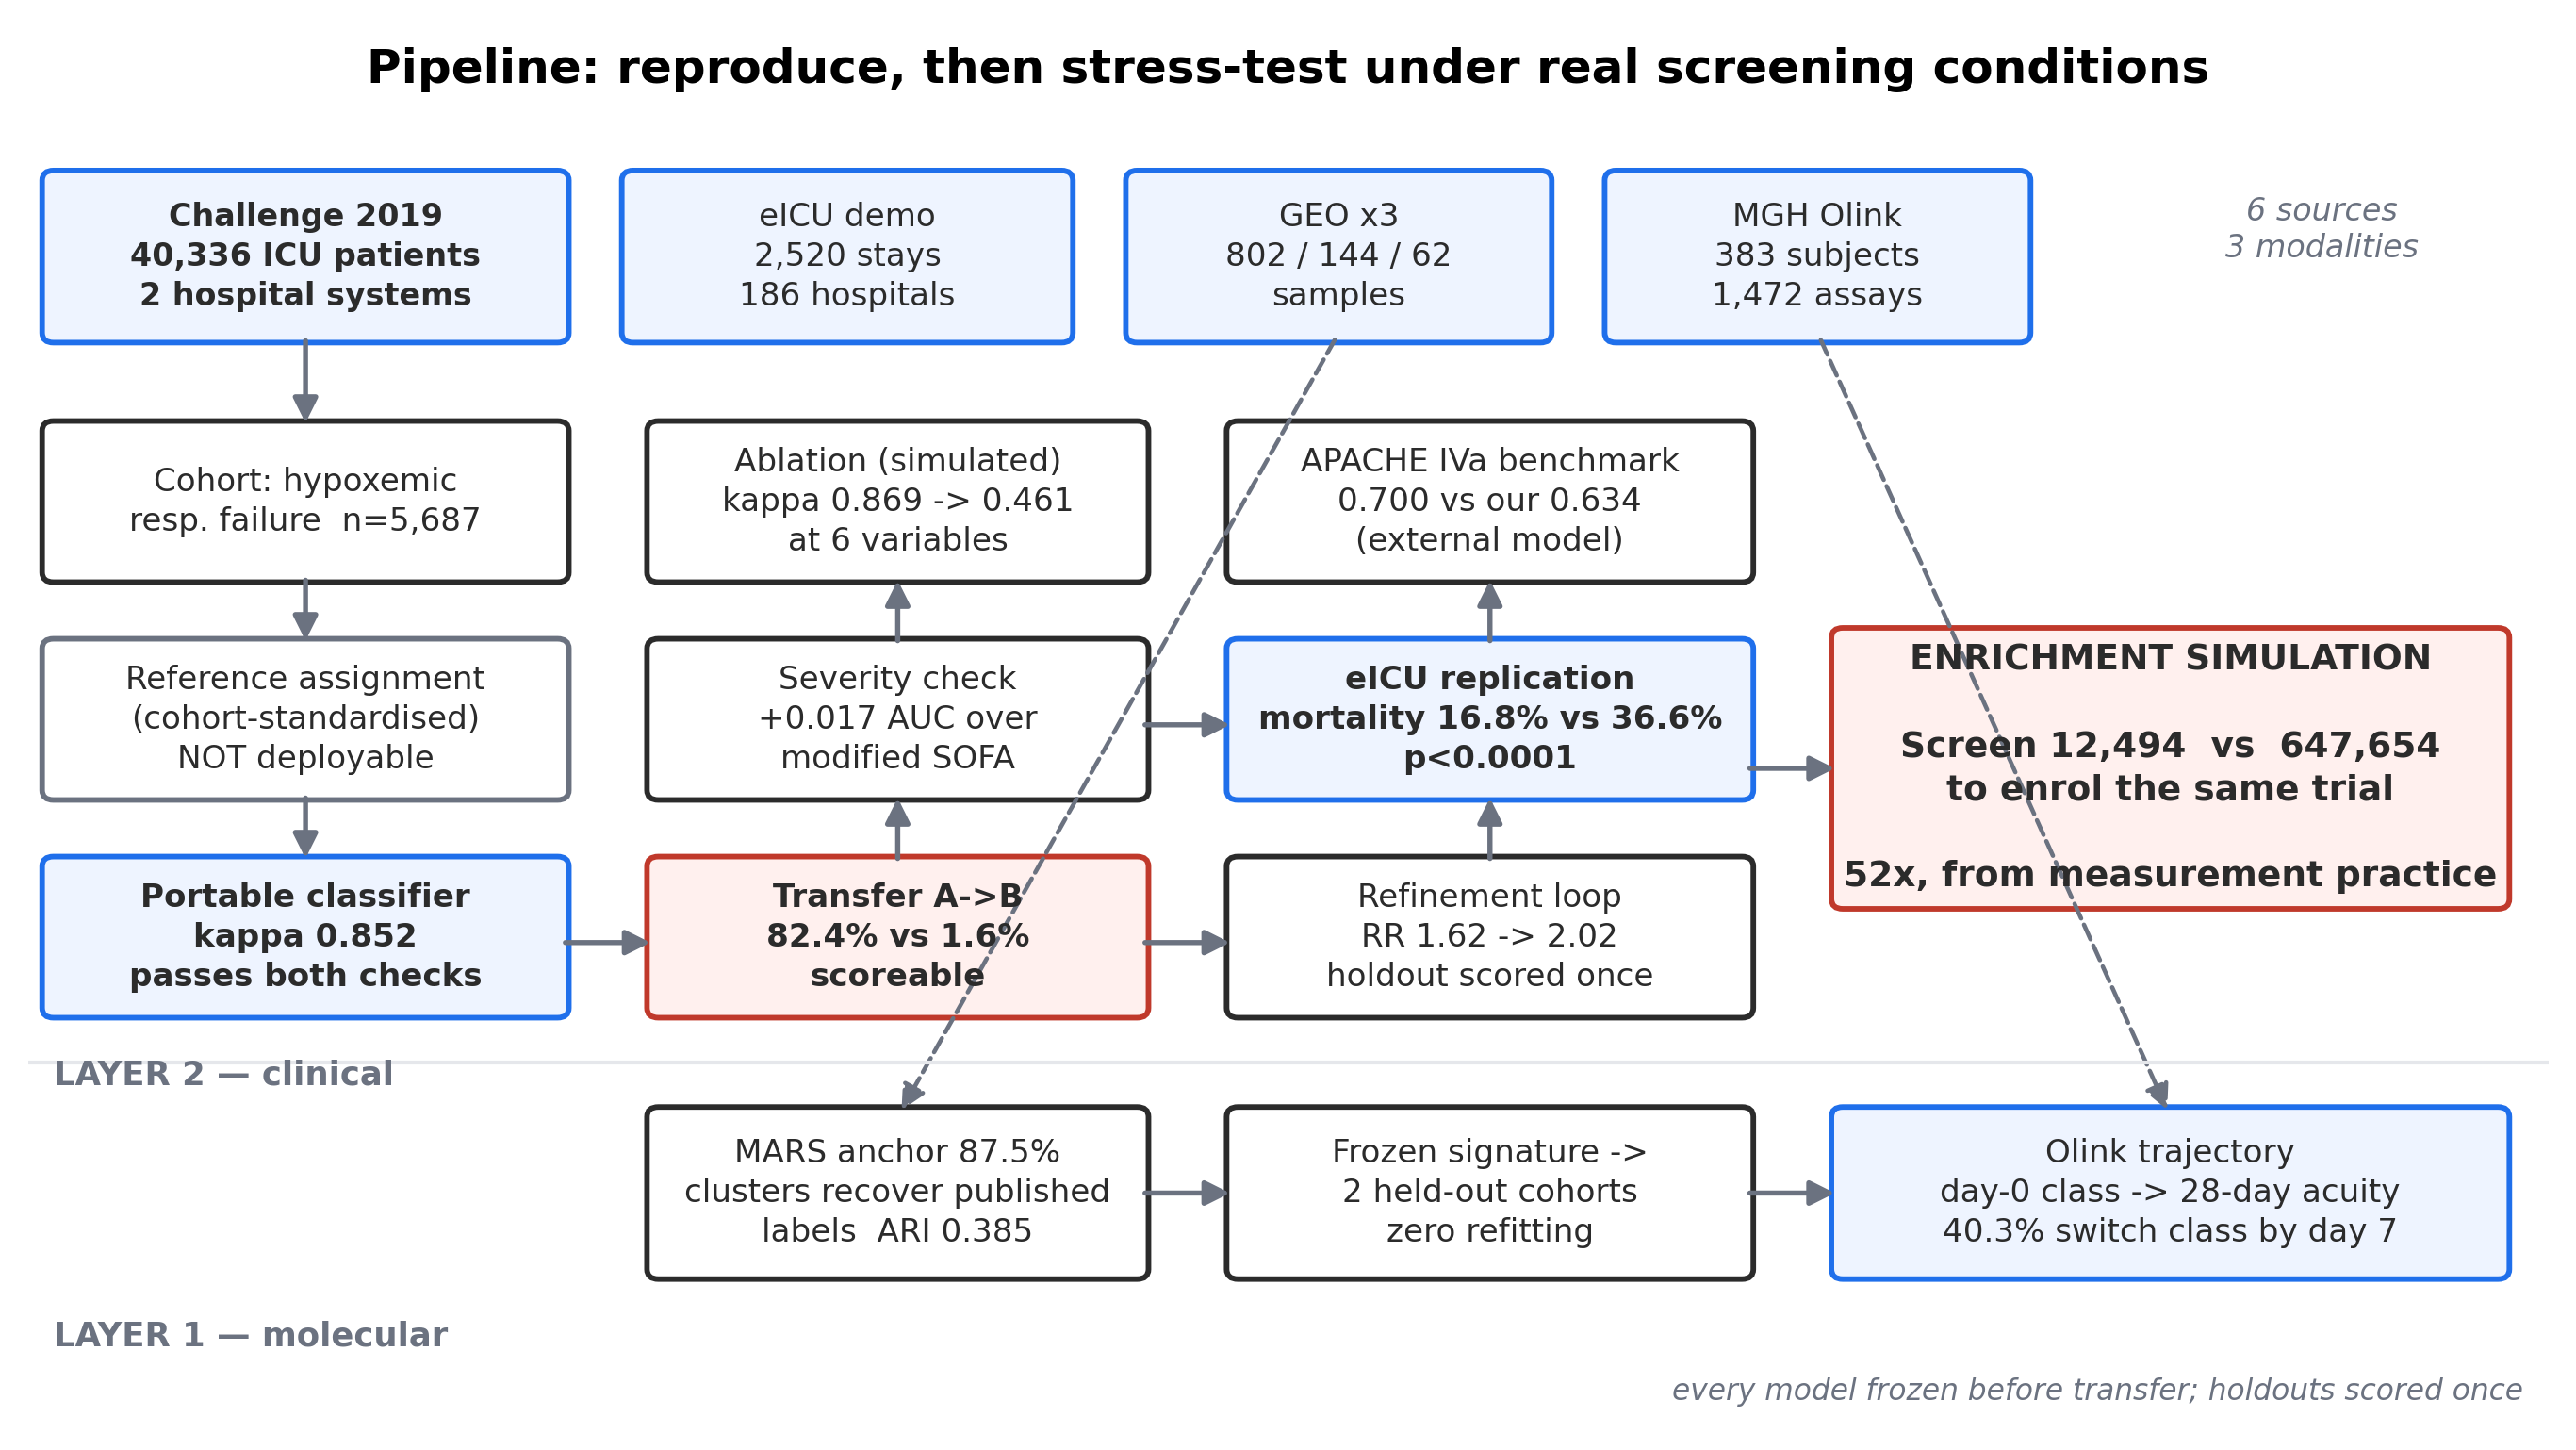
\includegraphics[width=\textwidth]{pipeline_overview.png}
  \caption{Analysis pipeline. Six sources, three modalities. Every model is frozen before it
  crosses a dataset boundary, and the refinement loop's holdout is scored exactly once}
  \label{fig:pipeline}
\end{figure}

\section{Methods}

\subsection{Data sources}

Six open-access sources were used (Table~\ref{tab:sources}). Attribution requirements are
met in \texttt{CITATIONS.md}.

\begin{table}[H]
\centering\small
\begin{tabular}{lll}
\toprule
Source & Size & Role \\
\midrule
PhysioNet/CinC Challenge 2019 & 40,336 patients, 2 systems & Primary cohort \\
eICU-CRD Demo & 2,520 unit stays & Mortality; external benchmark \\
MIMIC-IV Demo & 100 patients & Schema familiarity, smoke tests \\
GSE65682 (MARS) & 802 samples, 479 labelled & Transcriptomic discovery, anchor \\
GSE32707, GSE66890 & 144 and 62 samples & Transcriptomic transfer \\
MGH Olink Explore 1536 & 383 subjects, 1,472 assays & Proteomics, longitudinal \\
\bottomrule
\end{tabular}
\caption{Data sources}
\label{tab:sources}
\end{table}

\subsection{Cohort definition}

Berlin criteria cannot be approximated on this data path: there is no imaging, no PEEP and
no ventilation flag. The cohort is therefore \textbf{hypoxemic respiratory failure
identified by an \Spo/\Fio{} surrogate}, and is never described as ARDS. A pre-commit guard
enforces that wording mechanically.

Inclusion required age $\ge 18$, at least 24 hours of record, and at least one hour with
S/F $\le 235$ (a validated surrogate for P/F $\le 200$). Hours with \Spo$\,\ge 97$ were
excluded because the ratio is uninformative once the oximeter saturates, as were qualifying
hours beyond ICU hour 168. All thresholds were frozen before any data was read.

Observed \Fio{} ranged from 0.000 to 10.000 on a fraction scale where room air is 0.209;
321 of 112,155 values (0.29\,\%) are physiologically impossible. A validity window of
$[0.21, 1.0]$ was pre-registered. The errors are asymmetric --- a value above 1.0
\emph{deflates} S/F and would falsely admit a patient as severely hypoxemic --- which is why
they are filtered explicitly rather than dismissed as rare.

\subsection{Features and the treatment of missingness}

Static features summarise T0 to T0$+$24\,h; longitudinal features bin T0 to T0$+$72\,h into
twelve 6-hour intervals. \textbf{Every value channel carries a parallel binary mask}
recording whether the measurement was taken, because forward-filling without one fabricates
trajectories. Nothing is imputed at any point: cohort-median imputation would introduce a
population statistic into the inference path, which the portability checks of
Section~\ref{sec:portable} exist to forbid.

A third channel, \texttt{in\_record}, marks whether the patient was still in the ICU during
each bin. Without it the mask conflates \emph{not ordered} with \emph{already discharged}.
The distinction is large rather than pedantic: overall observation density is 27.2\,\% raw
but 52.5\,\% within the record, so nearly half of apparent missingness is censoring.

\subsection{Reference assignment, and what ``reproduction'' means here}

Four distinct objects are involved, and conflating them would overstate the result:
(1)~the \textbf{published} subphenotype structure, derived by latent class analysis on trial
cohorts \citep{calfee2014,famous2017,sinha2020lrm}; (2)~a \textbf{reference assignment}
fitted here, on this cohort, by Gaussian mixture; (3)~a \textbf{portable approximation} of
that reference assignment; and (4)~\textbf{external prognostic validation} of the portable
model in an independent database.

This study demonstrates that (2) recovers the \emph{directional pattern} of (1), that (3)
reproduces (2) at high agreement, and that (4) holds. It does \textbf{not} demonstrate that
(2) is the same partition as the published latent classes: published class assignments for
these patients do not exist, so no direct agreement can be computed. Where the text says
``recovered'' it means the directional pattern; ``reproduced'' means agreement with the
reference assignment fitted here.


A Gaussian mixture on log-transformed, \textbf{cohort-standardised} static features, fitted
on hospital system A. It requires the cohort mean and standard deviation of every variable
at inference and is therefore not deployable by construction. It exists to generate labels,
not to ship. $k$ was selected by BIC over a pre-registered range of 2--4 with 100 restarts.

\subsection{Portable classifiers and how portability was verified}
\label{sec:portable}

Three candidate forms --- logistic regression on raw values, a depth-4 decision tree with
absolute cut-points, and gradient boosting --- were trained to reproduce the reference
labels using only per-patient values. The portability claim is made \textbf{executable
rather than asserted}, by two independent checks:

\begin{enumerate}
\setlength{\itemsep}{1pt}
\item \emph{Static introspection} walks the fitted estimator and rejects any component
      carrying a cohort-derived statistic applied at transform time --- scalers, imputers,
      PCA.
\item \emph{Functional batch-invariance} predicts each patient alone and again inside the
      full batch and requires the two to be identical. This is the check that binds, because
      a model can pass introspection and still normalise inside a custom predict function.
\end{enumerate}

\subsection{Cross-hospital transfer}

Models fitted on system A were frozen and applied to system B with no refitting, under two
feature sets whose contrast isolates the mechanism: a \textbf{restricted} set of 14
variables whose coverage differs by less than 10 percentage points between sites, and a
\textbf{naive} set of 12 including the blood-gas block. Because system B contains no
patients with reference labels, transfer is evaluated by scoreability, predicted prevalence,
and whether the predicted class still stratifies sepsis onset --- an endpoint recorded
independently of whether the classifier can run.

\subsection{Severity comparison}
\label{sec:severity}

Severity is a \textbf{modified} SOFA, and must not be called SOFA. Two of six organ systems
are unavailable: cardiovascular is capped at 1 point for want of vasopressor dosing, and CNS
is omitted entirely for want of GCS. Maximum attainable score is 17 rather than 24, and
bilirubin is missing for 77\,\% of patients so the liver component scores zero by default
for most. Every one of these deficiencies weakens the severity score and therefore
\textbf{biases the comparison in the endotype's favour}.

\subsection{Ablation}

Three analyses. \textbf{(A)} Progressive removal of variables, ordered
least-available-first rather than least-important-first, because a deployment loses whatever
the site does not measure. \textbf{(B)} Natively sparse versus natively complete patients.
\textbf{(C)} A model trained on the missingness mask alone, with every value discarded.

Analyses B and C run on the full cohort against sepsis onset rather than on labelled
patients. This is not a convenience: endotype labels exist only for the reference model's
complete cases, within which the mask is all-ones by construction, so labelled patients
cannot support any question \emph{about} missingness (Section~\ref{sec:corrections}).

\subsection{Enrichment simulation}

Prognostic enrichment only --- a power calculation, not a causal claim. Given observed event
rates per class, required sample size was computed for unstratified enrollment and for
enrollment restricted to the higher-event-rate class, at 80\,\% power, $\alpha = 0.05$ and an
assumed 20\,\% relative risk reduction. Misclassification was modelled through positive
predictive value, and screening burden from the fraction of patients who can be scored at
all. \textbf{Predictive} enrichment --- which patients benefit more from treatment --- is a
different question requiring a treatment-effect estimate, is confounded by indication in
observational data, and was not attempted.

\subsection{Refinement loop}

One documented cycle. System B was split once with a fixed seed into a diagnosis slice and a
final holdout. Round 1 predicted on the diagnosis slice; errors were stratified by
missingness, age and predicted class into a taxonomy; refinements were selected by
\textbf{rules written down before any diagnosis ran}; round 2 was evaluated on the holdout,
scored exactly once.

\subsection{Molecular layer (secondary)}

\textbf{This layer is biological triangulation, not validation of the clinical classifier.}
The two cannot validate one another: the cohorts share no patients, the modalities differ,
and no patient-level link exists. It is included because it tests whether an inflammatory
two-class structure is recoverable in molecular data at all, and because the longitudinal
proteomics answer a question the clinical layer cannot --- whether class membership is stable
over time.

A regularised multinomial model was trained on GSE65682 to predict published MARS endotype
labels, with the resulting signature frozen. Consensus clustering with PAC-based $k$
selection was run independently. The frozen signature was scored on two held-out cohorts on
different array platforms with zero refitting; \textbf{cohorts were never merged}, since
merging across platforms manufactures clusters that separate by batch. Olink day-0 NPX was
clustered and related to a five-level acuity ordinal at days 0, 3, 7 and 28. Pathway sets
were pre-registered before any clustering ran.

\subsection{Pre-registration, guards and reproducibility}

Thresholds, feature sets and gene sets were committed before the analyses that use them, so
commit ordering makes the freeze auditable. Every extraction step carries an assertion
checkpoint with an expected row-count range. Pre-commit guards block row-level data,
discovery language, the ARDS-vocabulary violation and credential leaks. Thirty-three tests
cover the guards and the consensus-clustering implementation.

\section{Results}

\subsection{Cohort}

From 40,336 patients, 5,687 met criteria (4,680 in system A, 1,007 in system B;
Table~\ref{tab:attrition}). The cohort is selected rather than representative: requiring a
recorded \Fio{} picks out patients who are older, stay longer and have roughly triple the
sepsis rate, with standardised differences of 0.19 to 0.34. System B's cohort has a higher
baseline sepsis rate than system A's (22.2\,\% versus 13.9\,\%).

\subsection{The expected directional pattern is recovered}

At $k=2$, the class with the lowest bicarbonate showed \textbf{all four directions the
published literature reports} for the hyperinflammatory class --- lower bicarbonate, higher
creatinine, higher white cell count, higher event rate --- at a prevalence of 28.5\,\%,
inside the 20--35\,\% range published cohorts report. These four were specified in advance
as the directional signature to check; agreement with the published \emph{assignment} is not
computable, since published labels for these patients do not exist.

BIC preferred $k=4$. That value is the maximum of the pre-registered range with BIC still
falling, making it a \textbf{boundary solution}: the range, not the criterion, chose $k$. The
range was not widened afterwards, since doing so would be selecting $k$ by result.

\subsection{Portable classifiers reproduce the reference assignment}

\begin{table}[H]
\centering\small
\begin{tabular}{lrrr}
\toprule
Model & $\kappa$ & AUC & Brier \\
\midrule
Gradient boosting & 0.852 & 0.987 & 0.041 \\
Logistic regression & 0.723 & 0.932 & 0.082 \\
Decision tree (depth 4) & 0.671 & 0.871 & 0.093 \\
\bottomrule
\end{tabular}
\caption{Agreement with the reference assignment, out-of-fold. All three models passed both
portability checks}
\label{tab:portable}
\end{table}

The tree ships only split thresholds and is readable as a bedside rule. The parsimony curve
reaches its ceiling at four variables: BUN, bicarbonate, creatinine and pH. \textbf{Two of
those four are not recorded comparably at the second hospital.}

\subsection{Transfer is limited by measurement, not by the model}

\begin{table}[H]
\centering\small
\begin{tabular}{lrrr}
\toprule
Feature set & Variables & Scoreable, system A & Scoreable, system B \\
\midrule
Restricted (coverage-matched) & 14 & 79.8\,\% & \textbf{82.4\,\%} \\
Naive (includes blood gases) & 12 & 70.0\,\% & \textbf{1.6\,\%} \\
\bottomrule
\end{tabular}
\caption{Fraction of the cohort a frozen classifier can score at each site}
\label{tab:transfer}
\end{table}

The gap between 82.4\,\% and 1.6\,\% is measurement practice, isolated cleanly because the
restricted set's coverage is matched across sites by construction. Bicarbonate is recorded
for 97.4\,\% of system A patients and 2.1\,\% of system B; chloride 97.3\,\% versus
8.1\,\%; base excess 62.2\,\% versus 2.8\,\%. The difference runs in both directions ---
system B charts diastolic pressure (99.9\,\% versus 63.7\,\%) and troponin (32.8\,\% versus
2.4\,\%) \emph{more} (Figure~\ref{fig:coverage}) --- which identifies it as institutional measurement
behaviour rather than a data-quality defect at one site.

\begin{figure}[H]
  \centering
  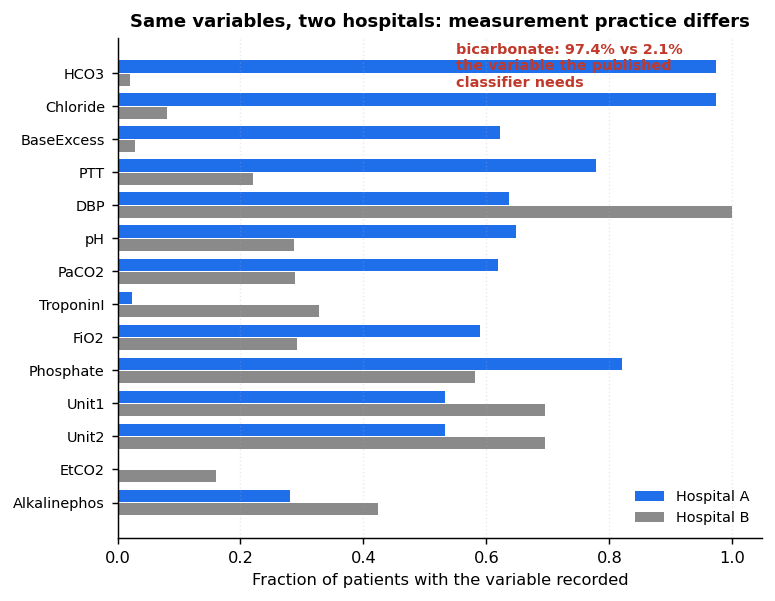
\includegraphics[width=0.75\textwidth]{coverage_by_hospital.png}
  \caption{Patient-level coverage for the variables differing most between the two hospital
  systems. The difference runs in both directions, which is why this is measurement practice
  rather than a defect at one site}
  \label{fig:coverage}
\end{figure}

\textbf{System B contains zero patients with reference labels.} Only 16 of its 1,007
cohort patients have the variables the reference model requires, so no site-native reference
assignment exists to compare against. The consequence bounds every transfer claim here:
\textbf{external transfer could be evaluated operationally and prognostically, but not by
direct label agreement.} Scoreability, predicted prevalence and outcome association are
measurable; external $\kappa$, sensitivity, specificity and calibration against a gold
assignment are not.

Predicted prevalence rose from 27.9\,\% at A to 35.2\,\% at B. The predicted class continued
to stratify sepsis onset in the same direction (22.9\,\% versus 18.0\,\%), but \textbf{not
significantly} ($p = 0.10$, overlapping intervals), where the same comparison at A was
decisive ($p < 0.0001$).

\subsection{Degradation, and a result that cuts against expectation}

Agreement fell from $\kappa = 0.869$ on 12 variables to 0.699 at 7, then to 0.461 at 6 and
0.130 at 2, losing half its full-feature performance by five variables
(Figure~\ref{fig:degradation}). Performance is comparatively flat from 12 down to 7 and
collapses thereafter.

\begin{figure}[H]
  \centering
  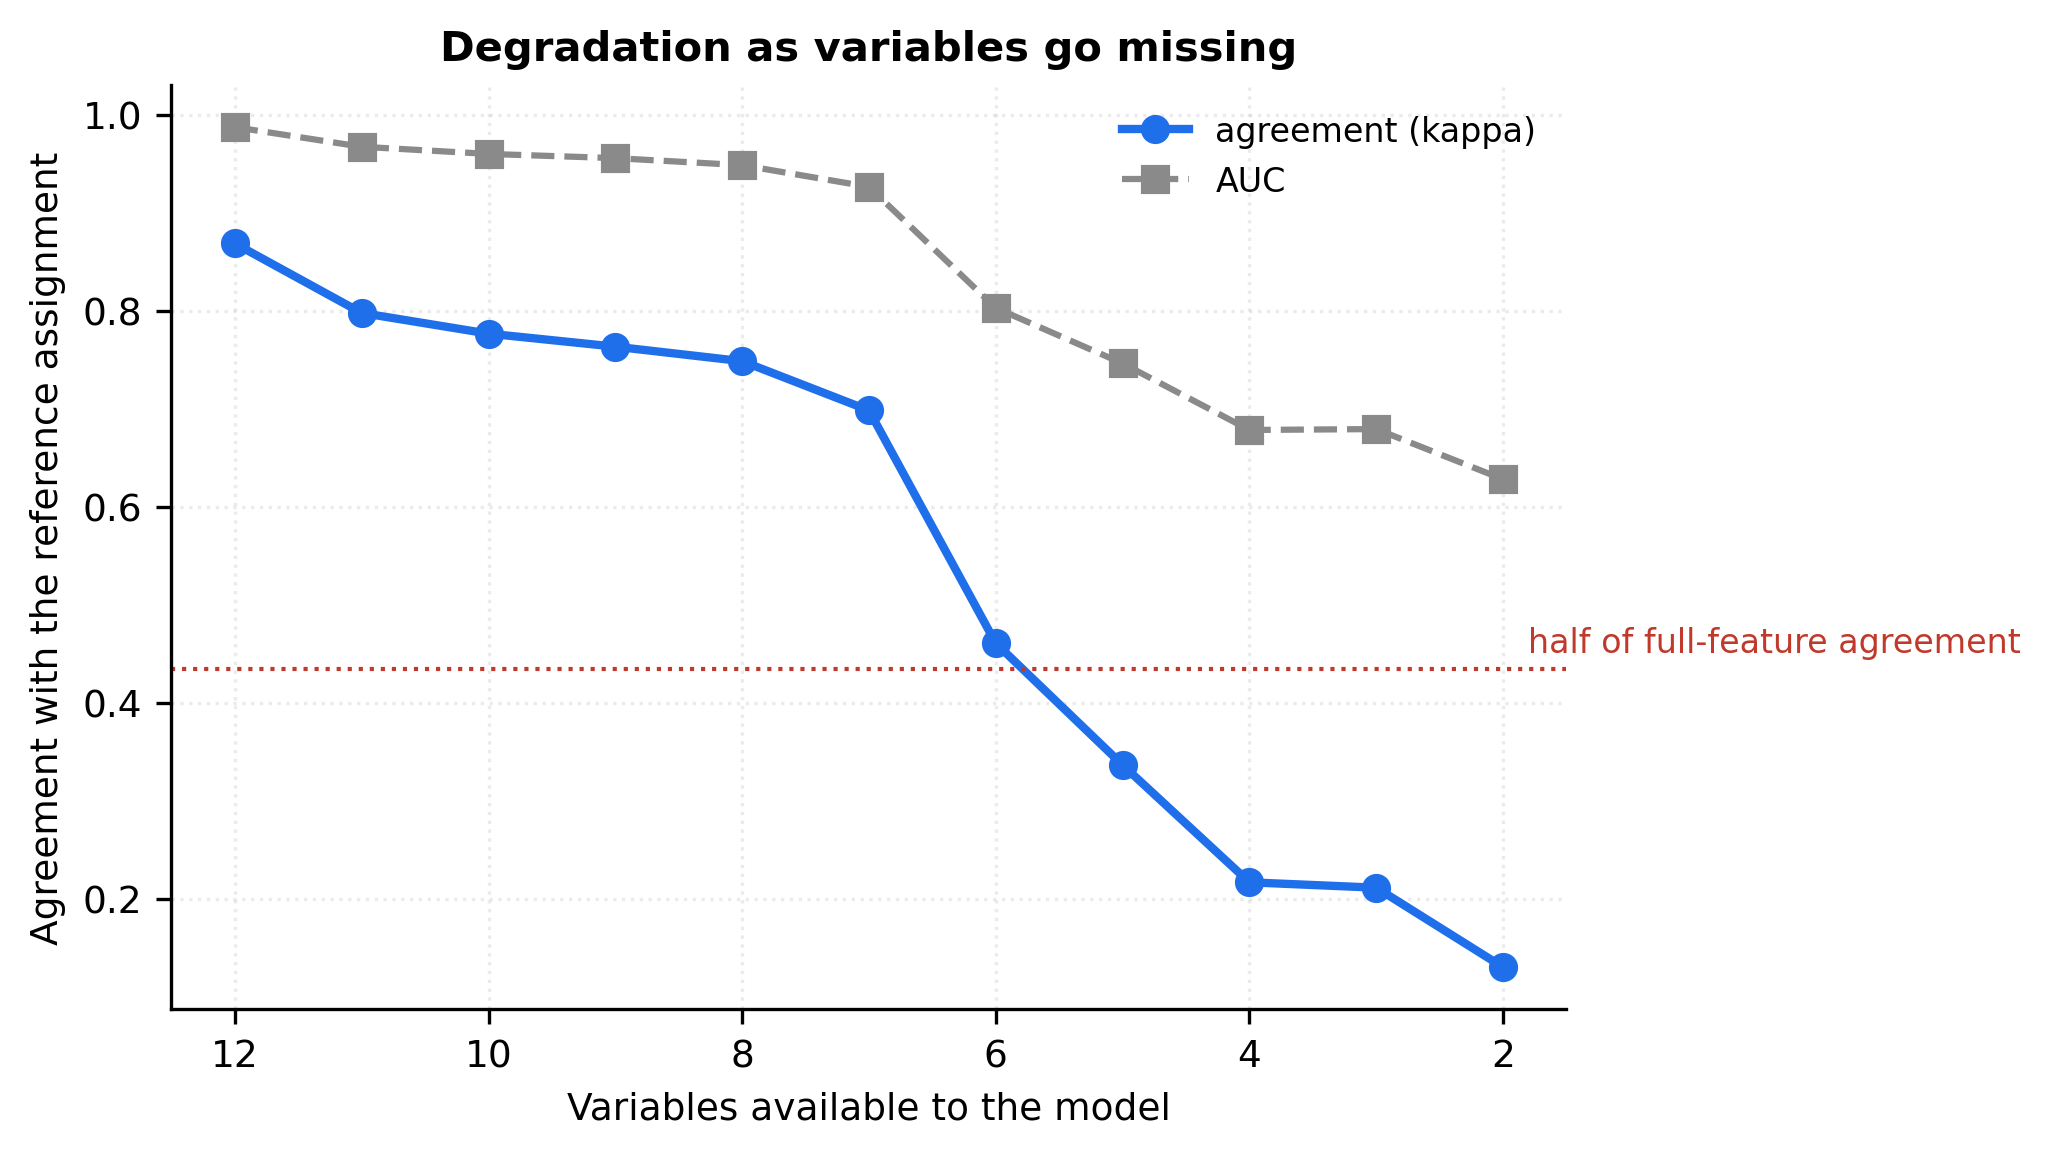
\includegraphics[width=0.85\textwidth]{degradation_curve.png}
  \caption{Agreement with the reference assignment as variables are removed
  least-available-first. The cliff falls between seven and six variables}
  \label{fig:degradation}
\end{figure}

Natively sparse patients ($n = 2{,}396$, mean 8.5 variables measured) have a \textbf{higher}
sepsis rate than the well measured (17.1\,\% versus 14.1\,\%, $n = 3{,}291$) and are
predicted \textbf{better} (AUC 0.675 versus 0.592). Sparse data is not degraded data here;
it marks a different kind of patient.

The missingness mask alone reached AUC 0.546 against 0.641 for the values, and added nothing
when combined with them (0.641 either way). Missingness therefore carries real but modest
signal, and the stronger conjecture that it might \emph{beat} the measurements is
\textbf{not supported}.

\subsection{The endotype adds little beyond the available severity score}

\begin{table}[H]
\centering\small
\begin{tabular}{lr}
\toprule
Predictor & AUC for sepsis onset \\
\midrule
Endotype alone & 0.544 \\
Modified SOFA alone & 0.540 \\
Both & 0.556 \\
\bottomrule
\end{tabular}
\caption{Endotype adds $+0.017$ AUC over severity, below the 0.02 threshold set before the
result was seen}
\label{tab:severity}
\end{table}

The endotype provided \textbf{little incremental discrimination beyond the available
severity score}. That phrasing is deliberate: the stronger claim that severity \emph{explains}
the classes is not supported, because the comparator is impaired and both predictors are
weak. Two qualifications prevent this being over-read. First, \textbf{all three values are
near chance}: severity does not predict sepsis onset either, so this compares two weak
predictors. Second, the severity score is deliberately weakened
(Section~\ref{sec:severity}), which biases the comparison toward the endotype and makes the
null \emph{stronger} than it appears. Classes partially survive severity adjustment: ARI
0.332 between the original assignment and one refitted with features standardised within
severity quartile. The confound is real but not total.

\subsection{Prognostic stratification replicates in an independent database}

Applying the frozen system-A model to the eICU demonstration database --- a different schema,
125 hospitals --- required mapping laboratory names and one unit conversion, since eICU
charts \Fio{} as a percentage where Challenge 2019 uses a fraction. All 14 transferable
features were present and passed range verification.

\begin{table}[H]
\centering\small
\begin{tabular}{lrrrr}
\toprule
Predicted class & $n$ & Deaths & Hospital mortality & 95\,\% CI \\
\midrule
Hypoinflammatory-like & 244 & 41 & 16.8\,\% & 12.3--22.1\,\% \\
Hyperinflammatory-like & 142 & 52 & 36.6\,\% & 28.7--45.1\,\% \\
\bottomrule
\end{tabular}
\caption{Mortality by predicted class in eICU. Fisher $p < 0.0001$, non-overlapping
intervals, a 2.2-fold ratio. What replicates is the mortality \emph{gradient}, not the
underlying biological endotype}
\label{tab:mortality}
\end{table}

\begin{figure}[H]
  \centering
  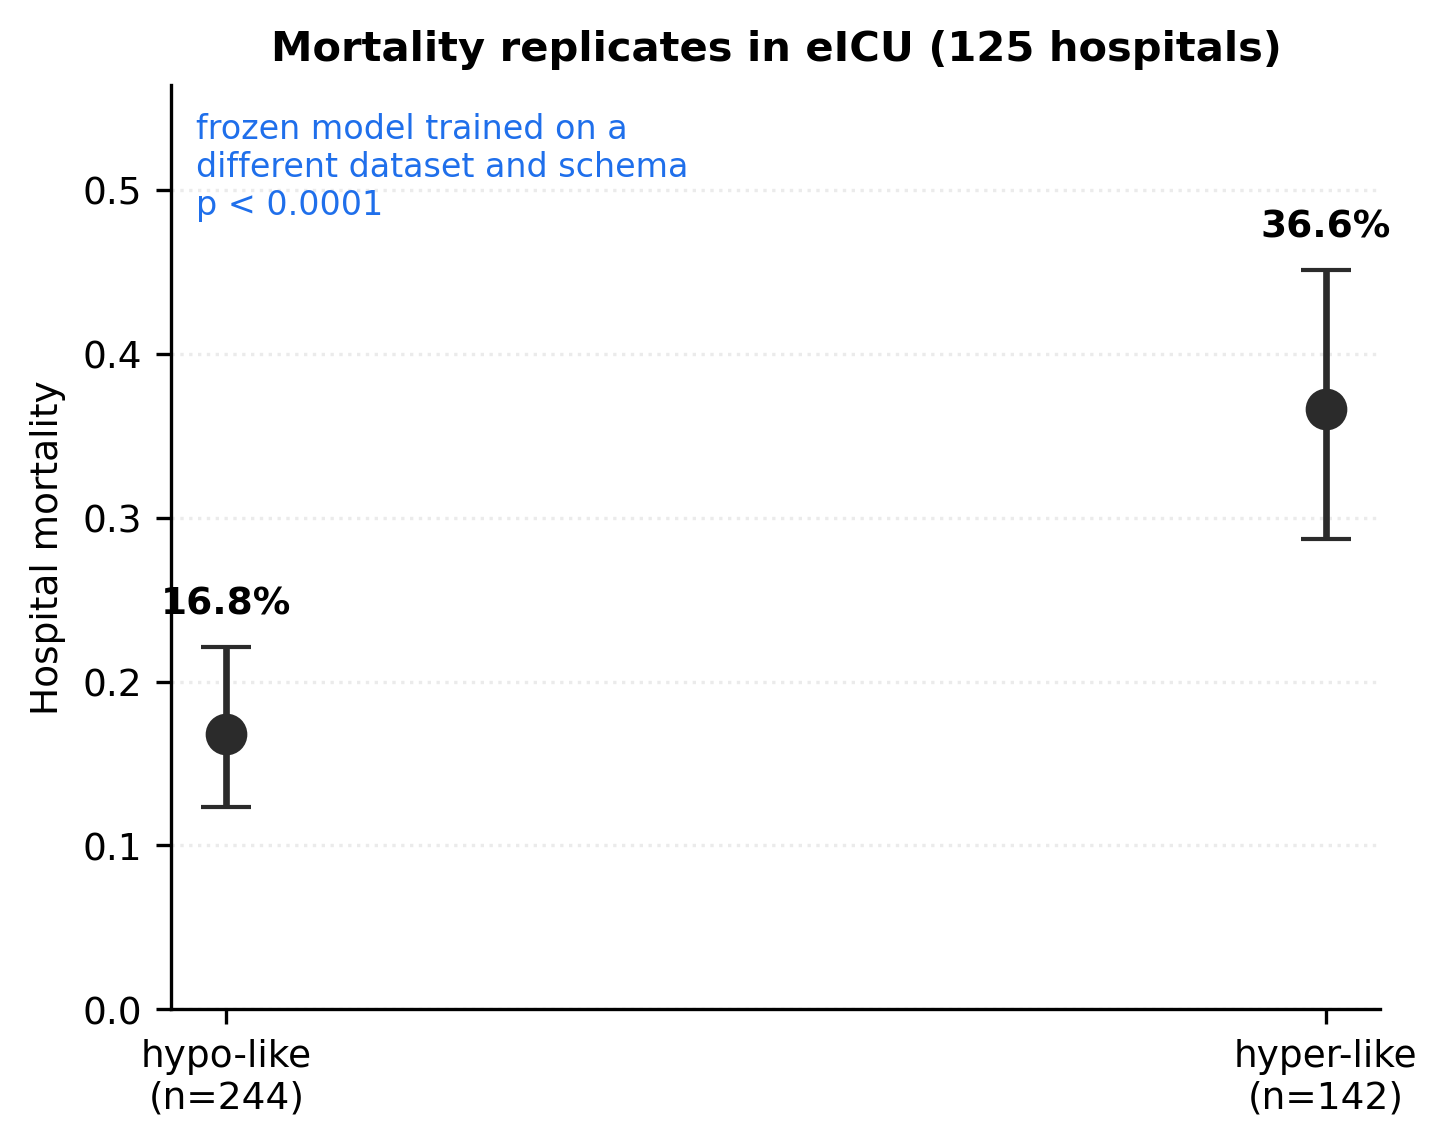
\includegraphics[width=0.60\textwidth]{eicu_mortality.png}
  \caption{Hospital mortality by predicted class, 95\,\% intervals. The model was trained on
  Challenge 2019 system A and frozen; eICU is a different dataset with a different schema}
  \label{fig:mortality}
\end{figure}

Benchmarked against APACHE IVa --- a published, externally validated model whose predictions
ship with the data and which was not fitted here --- the endotype probability reached AUC
0.634 against APACHE's 0.700. APACHE wins, as expected: it is purpose-built for mortality
prediction and an endotype label is not.

\subsection{Enrichment: the binding constraint is screening, not accuracy}

Unstratified enrollment requires 2,196 patients per arm; perfect enrichment on the
high-event class requires 1,573, a 28.4\,\% reduction; at realistic classifier accuracy,
1,798. \textbf{The trial size quoted below is $3{,}596 = 2 \times 1{,}798$}, both arms at
that accuracy.

Screening burden is where this becomes consequential. Patients must both test positive and
be scoreable at all, so the number screened is
$2n / (f_{\mathrm{pos}} \cdot f_{\mathrm{scoreable}})$, where $f_{\mathrm{pos}} = 0.349$ is
the fraction testing positive. To enrol the same 3,596 patients at the second hospital, the
coverage-matched model requires screening 12,494 patients and the blood-gas-dependent model
647,654 --- a 52-fold difference from an identical trial design
(Figure~\ref{fig:headline}).

\textbf{This ratio is more robust than it may appear.} Because trial size, accuracy,
prevalence and $f_{\mathrm{pos}}$ are identical in both rows, they cancel exactly, and the
ratio reduces to the scoreability ratio alone: $0.824 / 0.0159 = 51.8$. It therefore does not
depend on the assumed 20\,\% relative risk reduction, the 80\,\% power, or the assumed
classifier accuracy --- none of which enter the comparison. What it does depend on is the
observed coverage difference between the two hospitals.

\begin{figure}[H]
  \centering
  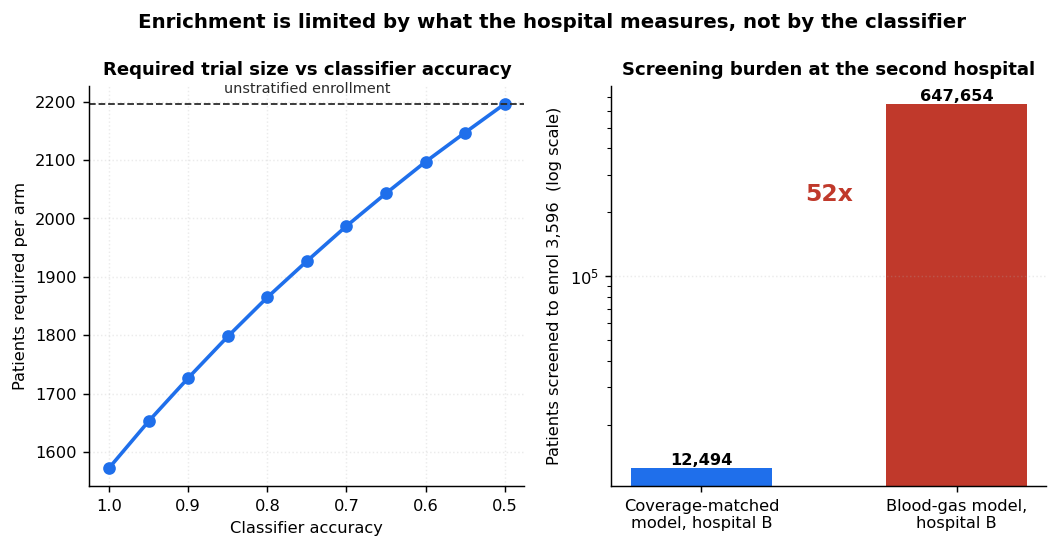
\includegraphics[width=\textwidth]{headline_enrichment.png}
  \caption{Left: required patients per arm as classifier accuracy falls, against unstratified
  enrollment. Right: patients who must be screened to enrol the same trial at the second
  hospital, coverage-matched versus blood-gas variables, log scale}
  \label{fig:headline}
\end{figure}

\subsection{Refinement}

The round-1 error taxonomy identified two concrete failure modes: the model is
\textbf{inverted} on sparsely measured patients (risk ratio 0.12 versus 1.71 on
well-measured), and the signal is carried almost entirely by patients aged 65 and over
(1.78 versus 0.98).

Two pre-specified rules fired: threshold recalibration, and the addition of
measured-variable count as an explicit feature. On the holdout, scored once, enrichment
improved (risk ratio 1.62 to 2.02, crossing into significance at $p = 0.039$) while
discrimination did not (AUC 0.634 to 0.629). This is the expected shape rather than a
contradiction, since both refinements act on the operating point and AUC is
threshold-invariant. \textbf{The deployable quantity improved; the model did not.}

\subsection{Molecular layer (secondary triangulation)}

The MARS endotype labels were present in GSE65682 metadata for 479 samples. A regularised
multinomial model predicted them at 87.5\,\% out-of-fold accuracy with per-class AUC 0.975
to 0.988. Consensus clustering, without access to those labels, partially recovered them
(ARI 0.385) --- but PAC remained at or above 0.42 at every $k$ searched, so \textbf{no
resolution gives a stable partition}, and the selected $k$ again sat at the range boundary.

The frozen signature scored on two held-out cohorts separated sepsis-with-ARDS from sepsis
alone in the expected direction but not significantly (Cliff's $\delta = +0.303$,
$p = 0.051$, $n = 29$ versus 28). In the longitudinal cohort, sepsis patients' scores rose
toward the ARDS level between day 0 and day 7 ($p = 0.024$) while ARDS patients started high
and stayed flat.

In Olink proteomics, day-0 class predicted acuity at every subsequent timepoint with the
effect \textbf{growing} over time (Cliff's $\delta$ from $-0.344$ at day 0 to $-0.505$ on
maximum acuity, all $p \le 10^{-6}$). \textbf{40.3\,\% of patients changed inflammatory
status between day 0 and day 7}, indicating states rather than fixed traits.

The p38 axis separated only marginally better than a disjoint generic-inflammation
comparator (Cliff's $\delta$ 0.676 versus 0.611, margin 0.065). An interferon negative
control showed no separation ($\delta = 0.002$, $p = 0.98$), confirming the comparison
detects pathway-specific signal rather than general activation. Per the pre-committed rule,
this is \textbf{consistent with, but not evidence of, p38-axis dominance}. Clusters did not
correspond to COVID status as a partition (ARI 0.053) but were not independent of it either
($\chi^2$, $p = 7 \times 10^{-18}$); the honest reading is partial host-response structure
with an aetiology component.

\section{Discussion}

\subsection{What each claim does and does not establish}

\begin{table}[H]
\centering\footnotesize
\begin{tabular}{p{0.29\textwidth}p{0.30\textwidth}p{0.33\textwidth}}
\toprule
Claim & Evidence & What it does \textbf{not} establish \\
\midrule
A two-class directional pattern is recoverable & GMM; four published directions at
28.5\,\% prevalence & That this partition equals the published latent classes \\
A portable classifier reproduces the reference assignment & $\kappa = 0.852$; both
portability checks passed & External classification accuracy at another site \\
The model transfers operationally & 82.4\,\% scoreable at system B & External label
agreement, calibration, sensitivity/specificity \\
Measurement practice limits deployment & 82.4\,\% vs 1.6\,\% scoreable; bicarbonate
97.4\,\% vs 2.1\,\% & Why each institution orders what it orders \\
The classes retain prognostic signal & eICU 16.8\,\% vs 36.6\,\% mortality,
$p<0.0001$ & Biological endotype replication; treatment-effect heterogeneity \\
Refinement improved enrichment & RR 1.62 $\rightarrow$ 2.02, holdout scored once &
Improved discrimination (AUC was flat) \\
\bottomrule
\end{tabular}
\caption{Claims, their evidence, and their bounds}
\label{tab:claims}
\end{table}


\textbf{The endpoint, not the classes, was the limiting factor.} On the primary cohort the
subphenotypes looked close to worthless: AUC 0.544 for sepsis onset, adding $+0.017$ over a
severity score. On eICU the same frozen model separated mortality by a factor of 2.2 with
$p < 0.0001$. Sepsis onset is a six-hour-shifted Sepsis-3 label these subphenotypes were
never derived against; mortality is what they were built on. Reporting either result without
the other would mislead, and the pairing is the single most important interpretive point in
this study.

\textbf{Deployability is governed by institutional measurement practice.} Not by
documentation quality: a variable absent from a record may never have been \emph{ordered},
which is a different and larger claim. The bidirectional difference supports the broader
reading --- system B records diastolic pressure and troponin more often, not less --- so what
differs is which tests each institution routinely obtains. The classifier is not the
bottleneck. A model reproducing its reference assignment at $\kappa = 0.852$ becomes
unusable at a hospital that does not order the tests it needs, and the parsimony curve makes
this worse rather than better: the most informative small variable set is disproportionately
built from blood-gas measurements, which are exactly the measurements whose ordering varies
most between institutions. Parsimony and portability pull in opposite directions.

\textbf{For trial design}, this reframes the enrichment question. The literature's attention
to classifier accuracy is reasonable but secondary; between a perfect classifier and a
realistic one the required trial size moves by a few hundred patients, whereas between two
real hospitals the screening burden moves by a factor of 52. A trial-feasibility assessment
that does not audit site-level variable coverage is measuring the wrong thing.

\textbf{On the sparse-patient result.} That patients with fewer measured variables have more
events and are predicted better is counterintuitive but not inexplicable: measurement
intensity encodes clinical trajectory, and the sparsely measured group likely mixes the
rapidly deteriorating with the briefly admitted. It is reported here as an observation
requiring explanation rather than as an explained finding.

\section{Limitations}

\begin{itemize}
\setlength{\itemsep}{1pt}
\item \textbf{The cohort is not ARDS.} No imaging, no PEEP, no ventilation flag; the
      definition rests on an oximetry surrogate in an unadjudicated population.
\item \textbf{The primary cohort has no mortality outcome.} Mortality rests entirely on 386
      eICU patients with 93 deaths --- thin, with intervals reported wide.
\item \textbf{The severity comparison is weakened by design}, missing vasopressors and GCS
      with bilirubin absent for 77\,\%. This biases toward the endotype, so the null is
      stronger than it appears, but it is not a like-for-like comparison with published SOFA
      analyses.
\item \textbf{The published biomarker classifier cannot be evaluated anywhere in this data.}
      IL-6 and sTNFR1 are absent from EHR data entirely; Olink NPX is a relative log2 scale
      rather than a concentration, so a fixed-coefficient equation cannot consume it; and the
      proteomic cohort's clinical file contains no bicarbonate. The model is implemented
      correctly and shown to be inapplicable, which is itself the finding.
\item \textbf{$k$ selection hit the pre-registered range boundary in both layers}, so the
      range rather than the criterion determined the number of classes in each case. This
      should not be read as establishing a four-class clinical solution or a six-class
      molecular one: BIC and PAC were both still improving at the edge of the searched
      range, so the preferred $k$ is unknown and may be larger. All substantive results use
      the two-class comparison, chosen for comparability with the published dichotomy rather
      than by the selection criterion.
\item \textbf{PAC never fell below 0.42} in the transcriptomic layer: no $k$ gives a stable
      partition, and the ARI against published labels is doing the work stability cannot.
\item The cohort is selected by its own inclusion criteria, and the reference-model subset is
      selected again by completeness --- a selection on a selection.
\item The proteomic cohort is COVID-era, so its inflammatory biology is related to but not
      identical with non-COVID acute respiratory failure.
\end{itemize}

\section{Methodological corrections}
\label{sec:corrections}

Six analyses in this study produced plausible-looking results that were wrong. Each was
caught by a test, an assertion or a range check rather than by inspection, and each is
recorded because the failure modes are more instructive than the successes.

\paragraph{An ablation that had conditioned away the thing it measured.}
The first missingness ablation reported every feature at 100\,\% availability and a
mask-only AUC of 0.499 --- which reads as ``missingness carries no signal.'' It does not.
Endotype labels exist only for the reference model's complete cases, so within the labelled
subset the mask is all-ones by construction and a model fitted on it cannot beat chance.
Caught by every availability printing as exactly 1.000. \emph{Any analysis of missingness
conducted on complete cases is answering a different question than it appears to.}

\paragraph{A comparator that overlapped the thing it was comparing against.}
The p38 protein set shared 7 of its 10 assays with the ``generic inflammation'' comparator,
so the finding that p38 separated better was substantially the set being compared with
itself. A circular comparison producing a \emph{positive} result is the most dangerous kind,
because nothing looks wrong. The comparator is now disjoint by construction.

\paragraph{One statistic reported where two disagreed.}
The host-response result was initially reported from ARI alone (0.053) while a chi-square on
the same table gave $p = 7 \times 10^{-18}$. These answer different questions --- whether
the partitions match, versus whether any dependence exists --- and a low ARI with a tiny $p$
means the clusters are not a relabelling of COVID status but some are enriched. The analysis
now requires both measures to agree before making the clean claim.

\paragraph{A substring match that swallowed the control group.}
In GSE66890 the exclusion label literally contains the phrase ``sepsis with ARDS'' --- the
full string reads ``not meeting the Berlin definition \ldots{} and that they were excluded
from analysis'' --- so a substring match folded five explicitly excluded patients into the
ARDS arm, inflating it from 29 to 34 and moving the effect size. Now matched exactly.

\paragraph{A time index that was not the index it appeared to be.}
An ingest checkpoint fired on 8,793 of 40,336 patients. ICULOS is perfectly contiguous for
every patient but 22\,\% \emph{start} after hour 1, because their record begins some hours
after admission. ICULOS is hours-since-admission; row position is not. The practical impact
was two patients out of 5,689 --- recorded anyway, because it is precisely the class of error
that shifts a variable amount per patient and never raises anything. The checkpoint that
caught it was written before the data was seen.

\paragraph{A clustering that was degenerate rather than unfavourable.}
The first consensus clustering used Euclidean distance with average linkage and returned one
478-patient cluster plus singletons, with ARI 0.0004. The method was changed to a
correlation distance, standard for expression data. \textbf{The distinction matters:} the
trigger was structural degeneracy --- singleton clusters, which the pre-specified criteria
already disqualify --- not an unfavourable agreement statistic. Changing method because a
result is disliked is result-chasing; changing it because the output is broken is diagnosis.

\paragraph{Two traps caught before they entered a result.}
eICU charts \Fio{} as a percentage where Challenge 2019 uses a fraction; missing this would
have made every S/F ratio a hundredfold too large and produced an empty cohort --- a failure
that would have looked like ``the cohort does not exist here'' rather than a units bug. And
the reference model's sTNFR1 coefficient in common circulation (1.1913) differs from the
value in the primary sources (1.1903); the difference is roughly 0.009 log-odds, flips no
classification, and would therefore have remained invisible indefinitely.

\section{What was not attempted, and why}

\textbf{Predictive enrichment.} Which patients \emph{benefit} more from treatment requires a
treatment-effect estimate and is confounded by indication in observational data. A causal
forest here would return a confident, wrong and dangerous-sounding answer. The appropriate
design is a target-trial emulation with negative-control outcomes and E-value sensitivity
analysis.

\textbf{Drug--disease signature mapping.} Out of scope, and it would require a molecular
layer stronger than the one obtained.

\textbf{Refitting the reference classifier on NPX.} Legitimate as an exercise, but the
resulting model would be ours rather than an external reference, and the entire design
depends on the reference being external.

\appendix
\section{Cohort attrition}

\begin{table}[H]
\centering\small
\begin{tabular}{lrrr}
\toprule
Step & System A & System B & Total \\
\midrule
All ICU patients & 20,336 & 20,000 & 40,336 \\
Age $\ge$ 18 & 20,336 & 19,978 & 40,314 \\
$\ge$ 24\,h of record & 15,837 & 14,809 & 30,646 \\
$\ge$ 1 valid S/F candidate hour & 6,470 & 2,078 & 8,548 \\
S/F $\le$ 235 (final cohort) & 4,680 & 1,007 & 5,687 \\
\bottomrule
\end{tabular}
\caption{CONSORT-style attrition by hospital system}
\label{tab:attrition}
\end{table}

\section{Reproducing this work}

\begin{verbatim}
conda env create -f environment.yml && conda activate ards
# see DOWNLOADS.md; data acquisition is manual by design
make test     # 33 tests, including the integrity guards
make scope    # descriptive scoping
\end{verbatim}

\sloppy
No data is committed. Every deviation from the original analysis plan is recorded in
\texttt{DECISIONS.md} with the observation that triggered it.

\begin{thebibliography}{99}

\bibitem{calfee2014}
C.~S. Calfee, K.~Delucchi, P.~E. Parsons, et al.
\newblock Subphenotypes in acute respiratory distress syndrome: latent class analysis of
data from two randomised controlled trials.
\newblock {\em Lancet Respir Med}, 2(8):611--620, 2014.

\bibitem{famous2017}
K.~R. Famous, K.~Delucchi, L.~B. Ware, et al.
\newblock ARDS subphenotypes respond differently to randomized fluid management strategy.
\newblock {\em Am J Respir Crit Care Med}, 195(3):331--338, 2017.

\bibitem{sinha2020lrm}
P.~Sinha, K.~L. Delucchi, D.~F. McAuley, et al.
\newblock Development and validation of parsimonious algorithms to classify ARDS phenotypes.
\newblock {\em Lancet Respir Med}, 8(3):247--257, 2020.
\newblock Coefficients used here are from supplementary appendix Table~S4, an
\emph{ancillary} model; the paper's headline three-variable model uses different variables.

\bibitem{sinha2020ajrccm}
P.~Sinha, M.~M. Churpek, and C.~S. Calfee.
\newblock Machine learning classifier models can identify ARDS phenotypes using readily
available clinical data.
\newblock {\em Am J Respir Crit Care Med}, 202(7):996--1004, 2020.

\bibitem{sinha2022}
P.~Sinha, K.~L. Delucchi, Y.~Chen, et al.
\newblock Latent class analysis-derived subphenotypes are generalisable to observational
cohorts of acute respiratory distress syndrome.
\newblock {\em Thorax}, 77(1):13--21, 2022.

\bibitem{reyna2020}
M.~A. Reyna, C.~S. Josef, R.~Jeter, et al.
\newblock Early prediction of sepsis from clinical data: the PhysioNet/Computing in
Cardiology Challenge 2019.
\newblock {\em Crit Care Med}, 48(2):210--217, 2020.

\bibitem{pollard2018}
T.~J. Pollard, A.~E.~W. Johnson, J.~D. Raffa, et al.
\newblock The eICU Collaborative Research Database.
\newblock {\em Sci Data}, 5:180178, 2018.

\bibitem{scicluna2017}
B.~P. Scicluna, L.~A. van Vught, A.~H. Zwinderman, et al.
\newblock Classification of patients with sepsis according to blood genomic endotype.
\newblock {\em Lancet Respir Med}, 5(10):816--826, 2017.

\bibitem{filbin2021}
M.~R. Filbin, A.~Mehta, A.~M. Schneider, et al.
\newblock Longitudinal proteomic analysis of severe COVID-19.
\newblock {\em Cell Rep Med}, 2(5):100287, 2021.

\bibitem{christie2015}
J.~D. Christie, S.~Vaslef, P.~K. Chang, et al.
\newblock A randomized dose-escalation study of the safety and anti-inflammatory activity of
the p38 MAPK inhibitor dilmapimod in severe trauma subjects at risk for ARDS.
\newblock {\em Crit Care Med}, 43(9):1859--1869, 2015.

\end{thebibliography}

\end{document}
